% arara: mkdir: {target: "out/tex"}
% arara: pdflatex: {draft: true, action: nonstopmode, options: "-recorder -file-line-error -output-dir=./out"}
% arara: pdflatex: {synctex: true, action: nonstopmode, options: "-recorder -file-line-error -output-dir=./out"}
\documentclass[a4paper]{article}
\usepackage{etex}

%%%% Math formatting
\usepackage{amsfonts} % Extra fonts for math formatting.
\usepackage{amsmath}
\usepackage{amsthm}
\usepackage{oz}

%%%% Graphical stuff.
\usepackage{array}
\usepackage{tikz}
\usetikzlibrary{shapes,arrows,decorations.pathmorphing,positioning}

%%%% Structural stuff
\usepackage{subcaption}

%%%% Leftanguage and font settings
\usepackage[T1]{fontenc} % Proper output encoding for diacritics, etc.
\usepackage{lmodern} % Quite a nice font.
\usepackage[UKenglish]{babel} % Basic language setting.
\usepackage[babel=true]{microtype} % Nicer looking text.
\usepackage[autostyle]{csquotes} % Better quoting.

%%%% Appearance
\usepackage{titling} % Better control over the title.
\usepackage{booktabs} % High-quality tables.
\usepackage{xcolor} % Easier handling of colors.

%%%% Title, author, etc.
\title{COMP3702 MDP Tutorial}
\author{Dimitri Klimenko}

%%%% Setup for the hyperref package.
\usepackage[bookmarks=true, pdfpagelabels]{hyperref} % Dynamic linking!
\hypersetup{
  pdftitle={\thetitle},
  pdfauthor={\theauthor},
  colorlinks,
  linkcolor={red!50!black},
  citecolor={blue!50!black},
  urlcolor={blue!80!black}
}

\newcommand{\R}{\mathbb{R}}
\newcommand{\expec}[1]{\mathbb{E} \left[{#1}\right]}
\DeclareMathOperator*{\argmin}{arg\,min}
\DeclareMathOperator*{\argmax}{arg\,max}

\newcommand{\stSpace}{\mathcal{S}}
\newcommand{\actSpace}{\mathcal{A}}
\newcommand{\transFunc}{T}
\newcommand{\rewFunc}{R}
\newcommand{\pol}{\pi}
\newcommand{\val}{V}



\newcolumntype{P}{%
>{\rule[-0.6cm]{0pt}{1.5cm}\centering$}p{1cm}<{$}}

\begin{document}

\maketitle

\section{Q3 from Tutorial 6/7}

\begin{figure}[h]
  \centering
  \caption{The environment}
  \label{fig:env}
  \begin{tabular}{|P|P|P|P|}
    \hline
    1 & 2 & 3 & 4 \tabularnewline
    \hline
  \end{tabular}
\end{figure}
A robot navigates in a very simple environment,
as shown in Figure~\ref{fig:env}.
Suppose the robot starts from cell 1 and tries to reach the goal state, which is
cell 4.
At each time step, the robot can attempt to move one cell to the left,
or one cell to the right.
However, due to control error, every time the robot moves,
it has an 80\% chance of ending up in its intended cell and also a 20\%
chance of staying where it is.
If the robot tries to move left from cell 1, it will simply stay in the
same place.
Each attempted move costs the robot 1 utilon,
while reaching the goal gives a reward of 10.

Please model the above navigation problem as an MDP with an infinite horizon and
discount factor $\gamma=0.95$.

\section{MDP model}
Our MDP model is $(\stSpace, \actSpace, \transFunc, \rewFunc, \gamma)$, where
\begin{itemize}
  \item $\stSpace$ is the state space.
  \item $\actSpace$ is the action space.
  \item $\transFunc$ is the transition function.
  \item $\rewFunc$ is the reward function.
  \item $\gamma = 0.95$ is the discount factor.
\end{itemize}

\subsection{State space}
Since the environment is static, we only need one state variable to fully
describe the problem state---the position of the robot.
As such, the state space for this problem can be represented as
$$\stSpace = \{s_1, s_2, s_3, s_4\}$$
As we've said that $s_4$ is a goal state, this implies that the
problem terminates once $s_4$ is reached.
There are multiple ways to do this, but for this problem we will represent
this by making $s_4$ a \emph{terminal state};
after the robot reaches this state it will no longer be able to take any
actions.
For the purposes of an MDP model, this will be equivalent to stating that
all actions will cause it to stay in $s_4$ and give zero reward.
Similarly, since we know that the agent starts in $s_0$, we can call
this state the \emph{initial state}---this would be the root of the tree
if we were using Monte-Carlo Tree Search to solve this problem.

\subsection{Action space}
The robot can only go left or right, so the action space for the problem is
simply
$$\actSpace = \{ Left, Right \}$$

\subsection{Transition function}
The transition function $\transFunc(s, a, s')$ describes the probabilities for
the possible next states $s'$, conditional on the robot being in state $s$
and taking action $a$,
i.e.
\begin{equation*}
\transFunc(s, a, s') = \Pr(S_{t+1}=s' \mid S_t=s, A_t=a)
\end{equation*}
where $S_t$ is the state at time $t$, and $A_t$ is the action at time $t$.
For this particular MDP model, we have
\begin{equation*}
T(s_4, Left, s_4) = T(s_4, Right, s_4) = 1
\end{equation*}
since we've stated that the game ends upon reaching $s_4$, so taking
either action from $s_4$ means that you stay there.
We also have
\begin{equation*}
T(s_1, Left, s_1) = 1
\end{equation*}
since moving left from $s_1$ causes us to stay in $s_1$.
Because the robot has an 80\% chance of going where it intended to go,
we have
\begin{gather*}
T(s_2, Left, s_1) =
T(s_3, Left, s_2) =
T(s_1, Right, s_2) =\\
T(s_2, Right, s_3) =
T(s_3, Right, s_4) = 0.8 .
\end{gather*}
Additionally, we have
\begin{gather*}
T(s_2, Left, s_2) =
T(s_3, Left, s_3) =
T(s_1, Right, s_1) =\\
T(s_2, Right, s_2) =
T(s_3, Right, s_3) = 0.2 ,
\end{gather*}
as the robot has a 20\% chance of staying in the same square when it
tries to move to a different one.
For all other transitions, we have
\begin{equation*}
  T(*, *, *) = 0 ,
\end{equation*}
because, for example, the robot can never end up in $s_3$ immediately
after being in $s_1$.

\begin{table}[h!]
  \caption{
    Transition matrix representation of $\transFunc$.
  }
  \label{tab:tm}
  \begin{subtable}{.5\linewidth}
    \centering
    \caption{Transition matrix $P_{Left}$}
    \label{tab:tm_left}
    \begin{tabular}{c|cccc}
            &$s_1$&$s_2$&$s_3$&$s_4$\\
      \hline
      $s_1$ & 1   & 0   & 0   & 0   \\
      $s_2$ & 0.8 & 0.2 & 0   & 0   \\
      $s_3$ & 0   & 0.8 & 0.2 & 0   \\
      $s_4$ & 0   & 0   & 0   & 1 \\
    \end{tabular}
  \end{subtable}
  \begin{subtable}{.5\linewidth}
    \centering
    \caption{Transition matrix $P_{Right}$}
    \label{tab:tm_right}
    \begin{tabular}{c|cccc}
            &$s_1$&$s_2$&$s_3$&$s_4$\\
      \hline
      $s_1$ & 0.2 & 0.8 & 0   & 0   \\
      $s_2$ & 0   & 0.2 & 0.8 & 0   \\
      $s_3$ & 0   & 0   & 0.2 & 0.8 \\
      $s_4$ & 0   & 0   & 0   & 1 \\
    \end{tabular}
  \end{subtable}
\end{table}

An alternative way to represent this information is with
\emph{transition matrices}, one for $Left$, and one for $Right$;
those matrices can be seen in Table~\ref{tab:tm}.
The rows of the transition matrix represent the \emph{current state} $s$,
and the columns represent the \emph{next state} $s'$.
For example, by looking at the cell in the second row and third column in
Table~\ref{tab:tm_right}, we can see that the probability of reaching
$s_3$ when going $Right$ from $s_2$ is 0.8,
i.e. $T(s_2, Right, s_3) = 0.8$.

\subsection{Reward function}
Since we have decided that $s_4$ is a \emph{terminal state}, we are
representing this by having the robot get ``stuck'' in $s_4$ after reaching
it.
This means that we must set the reward for taking actions from $s_4$ to
always be zero, or the robot could simply continue to collect rewards in
$s_4$ forever, as we're using an infinite-horizon MDP.
As such, we must instead give the robot a reward whenever it reaches
$s_4$.
We can't simply give the robot a reward for going $Right$ from $s_3$, as
sometimes the robot stays in $s_3$.
This means that our reward function $R$ needs to take the form
$$R(s, a, s') , $$
which represents the reward for reaching $s'$ after taking action $a$
from state $s$.

As we've said that the robot eternally recieves no rewards after $s_4$ is reached,
this means that
\begin{equation*}
  R(s_4, Left, s_4) = R(s_4, Right, s_4) = 0 .
\end{equation*}
The robot is given a reward of 10 reaching $s_4$;
we can also see by inspection of the trancition matrices that the only possible
way to reach $s_4$ is by going $Right$ from $s_3$.
Since it costs the robot $1$ utilon every time it moves, we have
\begin{equation*}
  R(s_3, Right, s_4) = 9 ,
\end{equation*}
which incorporates the reward for reaching $s_4$ as well as the move cost.
All other movements of the robot don't reach the goal but still cost one
utilon, so finally we have
\begin{equation*}
  R(*, *, *) = -1
\end{equation*}
for all other transitions.

\subsection{Graphical representation}
This MDP can also be represented via a graph, which can be seen in
Figure~\ref{fig:graph}.
The four blue nodes in the graph represent the various states, $s_1$, $s_2$,
$s_3$ and $s_4$,
while the arrows out of those nodes represent the actions ($Left$ and $Right$)
that can be taken from those states.
The filled black nodes are ``chance nodes'', representing
different possible outcomes due to a random event,
with labels like $p=0.2$ representing the probability $T(s, a, s')$ of
different state transitions.
The integer labels on the ends of the arrows represent the reward function
$R(s, a, s')$, which specifies the reward for reaching state $s'$ after
taking action $a$ from state $s$.

\begin{figure}
  \caption{A graphical representation of the MDP model}
  \label{fig:graph}
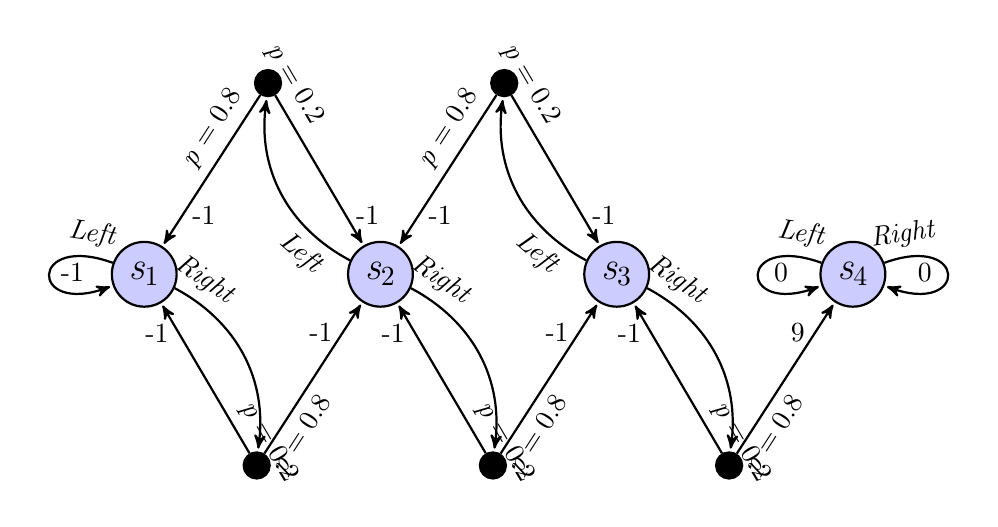
\begin{tikzpicture}[
    ->,>=stealth',shorten >=1pt,auto,node distance=3cm,thick,
  state/.style={circle,fill=blue!20,draw,font=\sffamily\Large\bfseries},
  chance/.style={circle,fill,draw,font=\sffamily\Large\bfseries},
]

  \node[state] (1) {$s_1$};
  \node[state] (2) [right of=1] {$s_2$};
  \node[state] (3) [right of=2] {$s_3$};
  \node[state] (4) [right of=3] {$s_4$};
  \node[chance] (2L) [above left =2cm and 1cm of 2] {};
  \node[chance] (3L) [above left =2cm and 1cm of 3] {};
  \node[chance] (1R) [below right=2cm and 1cm of 1] {};
  \node[chance] (2R) [below right=2cm and 1cm of 2] {};
  \node[chance] (3R) [below right=2cm and 1cm of 3] {};

  \draw [->] (1) to
    [out=160,in=200,looseness=10]
    node[above,sloped,pos=0.1]{$Left$}
    node[above,pos=0.8]{-1}
    (1);

  \draw [->] (2) to
    [bend left=35]
    node[below,sloped,pos=0.2]{$Left$} (2L);
  \draw [->] (2L) to
    node[sloped,pos=0]{$p=0.2$}
    node[right,pos=0.8]{-1}
    (2);
  \draw [->] (2L) to
    node[above,sloped,pos=0.3]{$p=0.8$}
    node[right,pos=0.8]{-1}
    (1);

  \draw [->] (3) to
    [bend left=35]
    node[below,sloped,pos=0.2]{$Left$} (3L);
  \draw [->] (3L) to
    node[sloped,pos=0]{$p=0.2$}
    node[right,pos=0.8]{-1}
    (3);
  \draw [->] (3L) to
    node[above,sloped,pos=0.3]{$p=0.8$}
    node[right,pos=0.8]{-1}
    (2);

  \draw [->] (1) to
    [bend left=35]
    node[sloped,pos=0.1]{$Right$} (1R);
  \draw [->] (1R) to
    node[sloped,pos=0]{$p=0.2$}
    node[left,pos=0.8]{-1}
    (1);
  \draw [->] (1R) to
    node[below,sloped,pos=0.2]{$p=0.8$}
    node[left,pos=0.8]{-1}
    (2);

  \draw [->] (2) to
    [bend left=35]
    node[sloped,pos=0.1]{$Right$} (2R);
  \draw [->] (2R) to
    node[sloped,pos=0]{$p=0.2$}
    node[left,pos=0.8]{-1}
    (2);
  \draw [->] (2R) to
    node[below,sloped,pos=0.2]{$p=0.8$}
    node[left,pos=0.8]{-1}
    (3);

  \draw [->] (3) to
    [bend left=35]
    node[sloped,pos=0.1]{$Right$} (3R);
  \draw [->] (3R) to
    node[sloped,pos=0]{$p=0.2$}
    node[left,pos=0.8]{-1}
    (3);
  \draw [->] (3R) to
    node[below,sloped,pos=0.2]{$p=0.8$}
    node[left,pos=0.8]{9}
    (4);

  \draw [->] (4) to
    [out=20,in=-20,looseness=10]
    node[above,sloped,pos=0.1]{$Right$}
    node[above,pos=0.8]{0}
    (4);

  \draw [->] (4) to
    [out=160,in=200,looseness=10]
    node[above,sloped,pos=0.1]{$Left$}
    node[above,pos=0.8]{0}
    (4);
\end{tikzpicture}
\end{figure}

\section{Policies and value functions}
\subsection{Policies}
A \emph{policy} $\pol : \stSpace \to \actSpace$ is a mapping from states to
actions.
This is the way we describe how the agent in an MDP will act;
in the context of a game we might also call this a \emph{strategy}.

If we associate the states with a specific order, we can also represent a
policy as an ordered list of actions \emph{tuple} that lists one action
for each state.
In this case, the obvious ordering is $(s_1, s_2, s_3, s_4)$,
and so an example policy is
\begin{equation*}
  \pol_L = (Left, Left, Left, Left) .
\end{equation*}
This is clearly not a very good policy because the robot's goal is to
get to the rightmost square, but it's a policy nonetheless!
A policy that's clearly better is
\begin{equation*}
  \pol_R = (Right, Right, Right, Right) ;
\end{equation*}
indeed, we will argue that this is one of two optimal policies in this MDP,
along with
\begin{equation*}
  \pol_2 = (Right, Right, Right, Left) ;
\end{equation*}

\subsection{Value functions}
A \emph{value function} $\val : \stSpace \to \R$ is a function that associates
each state with a \emph{value}, which is a real number that estimates, for
each state, how valuable it is for us to be in that state.
For example, a relatively silly value function would be
\begin{equation*}
  \val_0(\cdot) \equiv 0
\end{equation*}
which assumes that all states are equally worthless.

\subsection{The value of a policy}
For a given policy $\pol$ we can calculate the value function for
that policy $\val_\pol$ using equations that look like this:
\begin{equation} \label{eq:val}
  \val_\pol(s) = \sum_{s'} T(s, \pol(s), s') \bigg[ R(s, \pol(s), s') + \gamma \val_\pol(s') \bigg] ,
\end{equation}
where $s$ is the current state, $\pol(s)$ is the action that the policy
chooses for that state, and the values $s'$ represent the possible next states.
Since there many states, this actually forms a system of equations (one for each
state) that can be solved to calculate the value of a given policy.

Equation~\ref{eq:val} simply represents a calculation of the expected value
over different possibilities for the next state.
This is the sum of two terms:
the value of a given state is the expected value of the immediate reward,
\begin{equation} \label{eq:e_rew}
  \expec{R(s, a, \cdot)} = \sum_{s'} T(s, \pol(s), s') R(s, \pol(s), s')
\end{equation}
added to the discounted expected value of the next state,
\begin{equation}
  \gamma \sum_{s'} T(s, \pol(s), s') \val_\pol(s') .
\end{equation}
If the reward was independent of the next state, we could represent
our reward with a function $R(s, a)$ instead,
with $R(s, a, s') \equiv R(s, a)$.
Consequently, the expected reward over all possible next states
would simply be
\begin{equation*}
  \expec{R(s, \pol(s), \cdot)} \equiv R(s, \pol(s))
\end{equation*}
and Equation~\ref{eq:val} would
simplify to give
\begin{equation} \label{eq:val_rsa}
  \val_\pol(s) = R(s, \pol(s)) + \gamma \sum_{s'} T(s, \pol(s), s') \val_\pol(s') .
\end{equation}

\subsubsection{An example}
As an example, we can calculate the value of our not-very-good policy
\begin{equation*}
  \pol_L = (Left, Left, Left, Left) .
\end{equation*}
For convenience, we can turn Equation~\ref{eq:val} into a matrix form.
As you may recall, the transition function can represented by
\emph{transition matrices};
this also applies when we have a fixed policy.
Since $\pol_L$ says we should always go left, the appropriate transition
matrix is simply $P_L = P_{Left}$ from Table~\ref{tab:tm_left}, i.e.
\begin{equation*}
  P_L =
  \begin{pmatrix}
      1   & 0   & 0   & 0 \\
      0.8 & 0.2 & 0   & 0 \\
      0   & 0.8 & 0.2 & 0 \\
      0   & 0   & 0   & 1 \\
  \end{pmatrix}
\end{equation*}
Since moving left always has a cost of -1, we know that the expected
immediate reward will always be -1, except at $s_4$ where the reward
is always zero.
Consequently, we can represent the expected reward by the vector
\begin{equation*}
  \mathbf{r} = \begin{pmatrix}
    -1 \\ -1 \\ -1 \\ 0 \\
  \end{pmatrix} .
\end{equation*}
Using this, we can transform Equation~\ref{eq:val} to the matrix form
\begin{equation} \label{eq:val_matrix}
  \mathbf{v}_L = \mathbf{r} + \gamma P_L \mathbf{v}_L .
\end{equation}
I've switched to the notation $\mathbf{v}_L$ for the value function to
emphasize that it is a \emph{vector} in this equation.
Some basic algebra gives
\begin{equation*}
  (I - \gamma P_L) \mathbf{v}_L = \mathbf{r}
\end{equation*}
which is simply a system of linear equations in matrix form!
If we substitute the numbers in, we have
\begin{align*}
  \left[
    \begin{pmatrix}
      1 & 0 & 0 & 0 \\
      0 & 1 & 0 & 0 \\
      0 & 0 & 1 & 0 \\
      0 & 0 & 0 & 1 \\
    \end{pmatrix}
    - 0.95
    \begin{pmatrix}
      1   & 0   & 0   & 0 \\
      0.8 & 0.2 & 0   & 0 \\
      0   & 0.8 & 0.2 & 0 \\
      0   & 0   & 0   & 1 \\
    \end{pmatrix}
  \right]
  \mathbf{v}_L &=
  \begin{pmatrix}
    -1 \\ -1 \\ -1 \\ 0 \\
  \end{pmatrix} \\
  \begin{pmatrix}
    0.05  & 0     & 0    & 0    \\
    -0.76 & 0.81  & 0    & 0    \\
    0     & -0.76 & 0.81 & 0    \\
    0     & 0     & 0    & 0.05 \\
  \end{pmatrix}
  \begin{pmatrix}
    V_L(s_1) \\
    V_L(s_2) \\
    V_L(s_3) \\
    V_L(s_4)
  \end{pmatrix}
  &=
  \begin{pmatrix}
    -1 \\ -1 \\ -1 \\ 0 \\
  \end{pmatrix} \\
\end{align*}
If we solve the equations, we get
$$V_L(s_4) = 0 ,$$
and
$$V_L(s_1) = V_L(s_2) = V_L(s_3) = -20 .$$
This would mean that, from our initial state of $s_1$,
the expected value of our policy $\pol_L$ is -20.
Clearly not a very good policy\dots

\subsection{The one-step best policy for a value function}
Just as we calculated the value function for a given policy,
we can start with a value function and work out what the best
policy would be if those values were actually correct.
To make this simpler, we introduce the notion of a \emph{Q-value}, which
represents the estimated value of taking an action $a$ from state $s$.
The one-step Q-value for a given value function $V$ is, similarly to
Equation~\ref{eq:val},
\begin{equation}
  Q_V(s, a) = T(s, a, s') \bigg[ R(s, a, s') + \gamma \val(s') \bigg] ,
\end{equation}
Similarly, we can work out a \emph{one-step} best policy for a given
value function by looking one step ahead for every state, as per the above
equation, and choosing the action that has the best one-step value for
each state.
Consequently, the one-step best policy can be defined like this:
\begin{equation} \label{eq:best_pol}
  \pol(s) = \argmax_a Q_V(s, a) = \argmax_a \sum_{s'} T(s, a, s') \bigg[ R(s, a, s') + \gamma \val_\pol(s') \bigg] .
\end{equation}
which simply states that policy always takes the action that has the largest
expected value, when we look one step ahead with our given value function $V$.

\subsubsection{An example}
As an example, let's start with a value function $V_\sigma$ ($\sigma$ for silly), which
we will represent by the vector
\begin{equation*}
  \mathbf{v}_\sigma = (1, 0, 0, 0) .
\end{equation*}
In order to find the one-step best policy, we first calculate the values
of all the actions from looking one step ahead, which gives us the following:
\begin{align*}
  Q_\sigma(s_1, Left)  &= -1 + 1 &= 0 \\
  Q_\sigma(s_1, Right) &= -1 + 0.95 (0.8 \cdot 0 + 0.2 \cdot 1) &= -0.81 \\
  Q_\sigma(s_2, Left)  &= -1 + 0.95 (0.8 \cdot 1 + 0.2 \cdot 0) &= -0.24 \\
  Q_\sigma(s_2, Right) &= -1 + 0 &= -1 \\
  Q_\sigma(s_3, Left)  &= -1 + 0 &= -1 \\
  Q_\sigma(s_3, Right) &= 0.8 \cdot (9 + 0.95 * 0) &= \\
  Q_\sigma(s_4, Left)  &= 0 + 0 &= 0 \\
  Q_\sigma(s_4, Right) &= 0 + 0 &= 0 \\
\end{align*}


\subsection{Optimal policies and optimal value functions}

\section{Value iteration}

\section{Policy iteration}

\end{document}
